\documentclass[10pt,aspectratio=169]{beamer}

\usetheme[numbering=fraction,progressbar=frametitle]{metropolis}
\usefonttheme{professionalfonts}
\usepackage[UTF8]{ctex}
\usepackage{appendixnumberbeamer}
\usepackage{amsmath,amssymb,bm}
\usepackage{booktabs}
\usepackage{graphicx}
\usepackage{multicol}
\usepackage{array}

\title{Shape Function Generator}
\subtitle{方法设计、结构约束与首轮实验结果}
\author{shape\_function-main}
\date{\today}

\newcommand{\xq}{\mathbf{x}_q}
\newcommand{\Xnode}{\mathbf{X}_i}
\newcommand{\ri}{\mathbf{r}_i}
\newcommand{\rhat}{\hat{\mathbf{r}}_i}
\newcommand{\phii}{\phi_i(\mathbf{x}_q)}
\newcommand{\phiref}{\phi_i^{\mathrm{ref}}(\mathbf{x}_q)}

\begin{document}

\maketitle

\begin{frame}{问题定义}
  \begin{columns}[T,onlytextwidth]
    \column{0.54\textwidth}
      \textbf{目标}：给定局部 patch，直接生成查询点处的 meshfree shape function
      \vspace{0.6em}

      \[
      \mathcal{G}_{\theta}:
      \left(
      \xq,\{\Xnode\}_{i=1}^{k},\beta,\rho_q
      \right)
      \mapsto
      \{\phii\}_{i=1}^{k}
      \]

      \begin{itemize}
        \item 输入不是全局场，而是 \alert{query-centered local patch}
        \item 输出不是位移/应力，而是 \alert{shape function weights}
        \item 目标是给 meshfree 求解器提供 \alert{快速近似或 warm start}
      \end{itemize}

    \column{0.43\textwidth}
      \begin{block}{核心约束}
        \[
        \sum_i \phi_i = 1
        \qquad
        \sum_i \phi_i \Xi = \xq
        \]
      \end{block}

      \begin{alertblock}{为什么难}
        patch 几何分布不规则\\
        支撑域尺度变化明显\\
        病态 patch 易导致矩条件恶化
      \end{alertblock}
  \end{columns}
\end{frame}

\begin{frame}{方法总览}
  \[
  \left(\xq,\{\Xnode\},\beta,\rho_q\right)
  \xrightarrow{\text{feature construction}}
  \{\mathbf{f}_i\}
  \xrightarrow{\text{backbone}}
  \{l_i\}
  \xrightarrow{\text{B1--B4 head}}
  \{\phi_i\}
  \]

  \vspace{0.6em}
  \begin{columns}[T,onlytextwidth]
    \column{0.48\textwidth}
      \begin{block}{Backbone 职责}
        \begin{itemize}
          \item 提取 patch 局部几何模式
          \item 学习 reference max-ent 的隐式算子映射
          \item 输出未约束 raw logits
        \end{itemize}
      \end{block}
    \column{0.48\textwidth}
      \begin{block}{Head 职责}
        \begin{itemize}
          \item 加入 locality 与 positivity bias
          \item 强化 partition of unity
          \item 用 reproducing correction 保证一阶一致性
        \end{itemize}
      \end{block}
  \end{columns}

  \begin{center}
    \small
    patch $\rightarrow$ 几何编码 $\rightarrow$ 算子 backbone $\rightarrow$ 结构保持输出头
  \end{center}
\end{frame}

\begin{frame}{局部几何编码}
  \begin{columns}[T,onlytextwidth]
    \column{0.56\textwidth}
      \[
      \ri = \Xnode - \xq,
      \qquad
      r_{\max} = \max_i \|\ri\|,
      \qquad
      \rhat = \frac{\ri}{r_{\max}}
      \]

      \[
      \mathbf{f}_i =
      \left[
      \rhat,\;
      \|\rhat\|,\;
      \beta,\;
      \rho_q
      \right]
      \]

      \begin{itemize}
        \item \textbf{query-centered}：去掉平移自由度
        \item \textbf{scale normalization}：把不同 patch 拉回统一尺度
        \item \textbf{$\rho_q$}：编码局部密度、各向异性、复杂度
      \end{itemize}

    \column{0.40\textwidth}
      \begin{alertblock}{当前实现的 locality 修正}
        Backbone 仍使用 $r_{\max}$ 做归一化，\\
        但 B2 window 改为
        \[
        r_{\mathrm{support}} = \alpha r_{\max},
        \qquad \alpha = 1.05
        \]
        避免最远邻居被系统性压到 0。
      \end{alertblock}
  \end{columns}
\end{frame}

\begin{frame}{Kernel-Operator Backbone}
  \begin{columns}[T,onlytextwidth]
    \column{0.57\textwidth}
      \[
      \mathbf{h}_i^{(0)} = \mathrm{MLP}_{\mathrm{lift}}(\mathbf{f}_i)
      \]

      \[
      \mathbf{g}_{ij}^{(\ell)} =
      \left[
      \mathbf{h}_i^{(\ell)}-\mathbf{h}_j^{(\ell)},
      \hat{\mathbf{r}}_i,\hat{\mathbf{r}}_j,
      \|\hat{\mathbf{r}}_i-\hat{\mathbf{r}}_j\|
      \right]
      \]

      \[
      \alpha_{ij}^{(\ell)} =
      \mathrm{softplus}\!\left(\mathrm{MLP}_{\mathrm{mod}}(\mathbf{g}_{ij}^{(\ell)})\right)
      \cdot
      w_{\mathrm{Wendland}}(\|\hat{\mathbf{r}}_i-\hat{\mathbf{r}}_j\|)
      \]

      \[
      \mathbf{h}_i^{(\ell+1)} =
      \mathbf{h}_i^{(\ell)} +
      \sum_j \bar{\alpha}_{ij}^{(\ell)} \mathbf{V}^{(\ell)}\mathbf{h}_j^{(\ell)}
      \]

    \column{0.39\textwidth}
      \begin{block}{设计动机}
        \begin{itemize}
          \item 对 node set 保持排列无关
          \item 用几何差分特征表达局部相对关系
          \item 用核调制强化 meshfree 邻域归纳偏置
        \end{itemize}
      \end{block}

      \begin{exampleblock}{对照组}
        MLP baseline 只做距离排序后的拼接映射，\\
        用来回答：\alert{几何算子偏置是否真的有价值？}
      \end{exampleblock}
  \end{columns}
\end{frame}

\begin{frame}{Structure-Preserving Head}
  \begin{columns}[T,onlytextwidth]
    \column{0.58\textwidth}
      \textbf{B1 Softplus}
      \[
      \phi_i^{(1)} = \mathrm{softplus}(l_i)
      \]

      \textbf{B2 Window modulation}
      \[
      \phi_i^{(2)} = \phi_i^{(1)}
      \cdot
      w\!\left(\frac{\|\ri\|}{r_{\mathrm{support}}}\right)
      \]

      \textbf{B3 Normalization}
      \[
      \phi_i^{\mathrm{base}} =
      \frac{\phi_i^{(2)}}{\sum_j \phi_j^{(2)} + \varepsilon}
      \]

      \textbf{B4 Reproducing correction}
      \[
      \phi_i =
      \phi_i^{\mathrm{base}}
      +
      \phi_i^{\mathrm{base}}
      \mathbf{p}_i^\top
      \mathbf{M}^{-1}
      \left(
      \mathbf{b} - \sum_j \phi_j^{\mathrm{base}}\mathbf{p}_j
      \right)
      \]

    \column{0.38\textwidth}
      \begin{block}{每一步保证什么}
        \begin{itemize}
          \item B1：平滑正值 bias
          \item B2：局部支撑与边界衰减
          \item B3：先恢复 POU
          \item B4：再恢复一阶重构
        \end{itemize}
      \end{block}

      \begin{alertblock}{关键点}
        B4 之后 \textbf{不能再归一化}，\\
        否则会破坏刚恢复的一阶一致性。
      \end{alertblock}
  \end{columns}
\end{frame}

\begin{frame}{Teacher 与训练目标}
  \begin{columns}[T,onlytextwidth]
    \column{0.56\textwidth}
      \textbf{Patch-level max-ent teacher}
      \[
      z_i = w_i \exp(-\ri^\top \bm{\lambda}),
      \qquad
      \phiref = \frac{z_i}{\sum_j z_j}
      \]

      Gaussian prior:
      \[
      w_i = \exp\!\left(
      -\beta \left(\frac{\|\ri\|}{r_{\max}}\right)^2
      \right)
      \]

      \vspace{0.4em}
      \textbf{训练目标}
      \[
      \mathcal{L} =
      \mathcal{L}_{\mathrm{data}}
      +
      \lambda_{\mathrm{cons}}\mathcal{L}_{\mathrm{cons}}
      +
      \lambda_{\mathrm{neg}}\mathcal{L}_{\mathrm{neg}}
      \]

      \[
      \mathcal{L}_{\mathrm{cons}} =
      \left(\sum_i \phi_i - 1\right)^2
      +
      \left\|
      \sum_i \phi_i \Xnode - \xq
      \right\|^2
      \]

    \column{0.40\textwidth}
      \begin{block}{角色定位}
        teacher 是 \alert{reference-guided warm start}，\\
        不是最终物理求解器替代品。
      \end{block}

      \begin{exampleblock}{监控指标}
        \begin{itemize}
          \item relative L2
          \item POU residual
          \item linear residual
          \item negative fraction
          \item cond($M$)
        \end{itemize}
      \end{exampleblock}
  \end{columns}
\end{frame}

\begin{frame}{首轮结果：训练与主指标}
  \begin{columns}[T,onlytextwidth]
    \column{0.57\textwidth}
      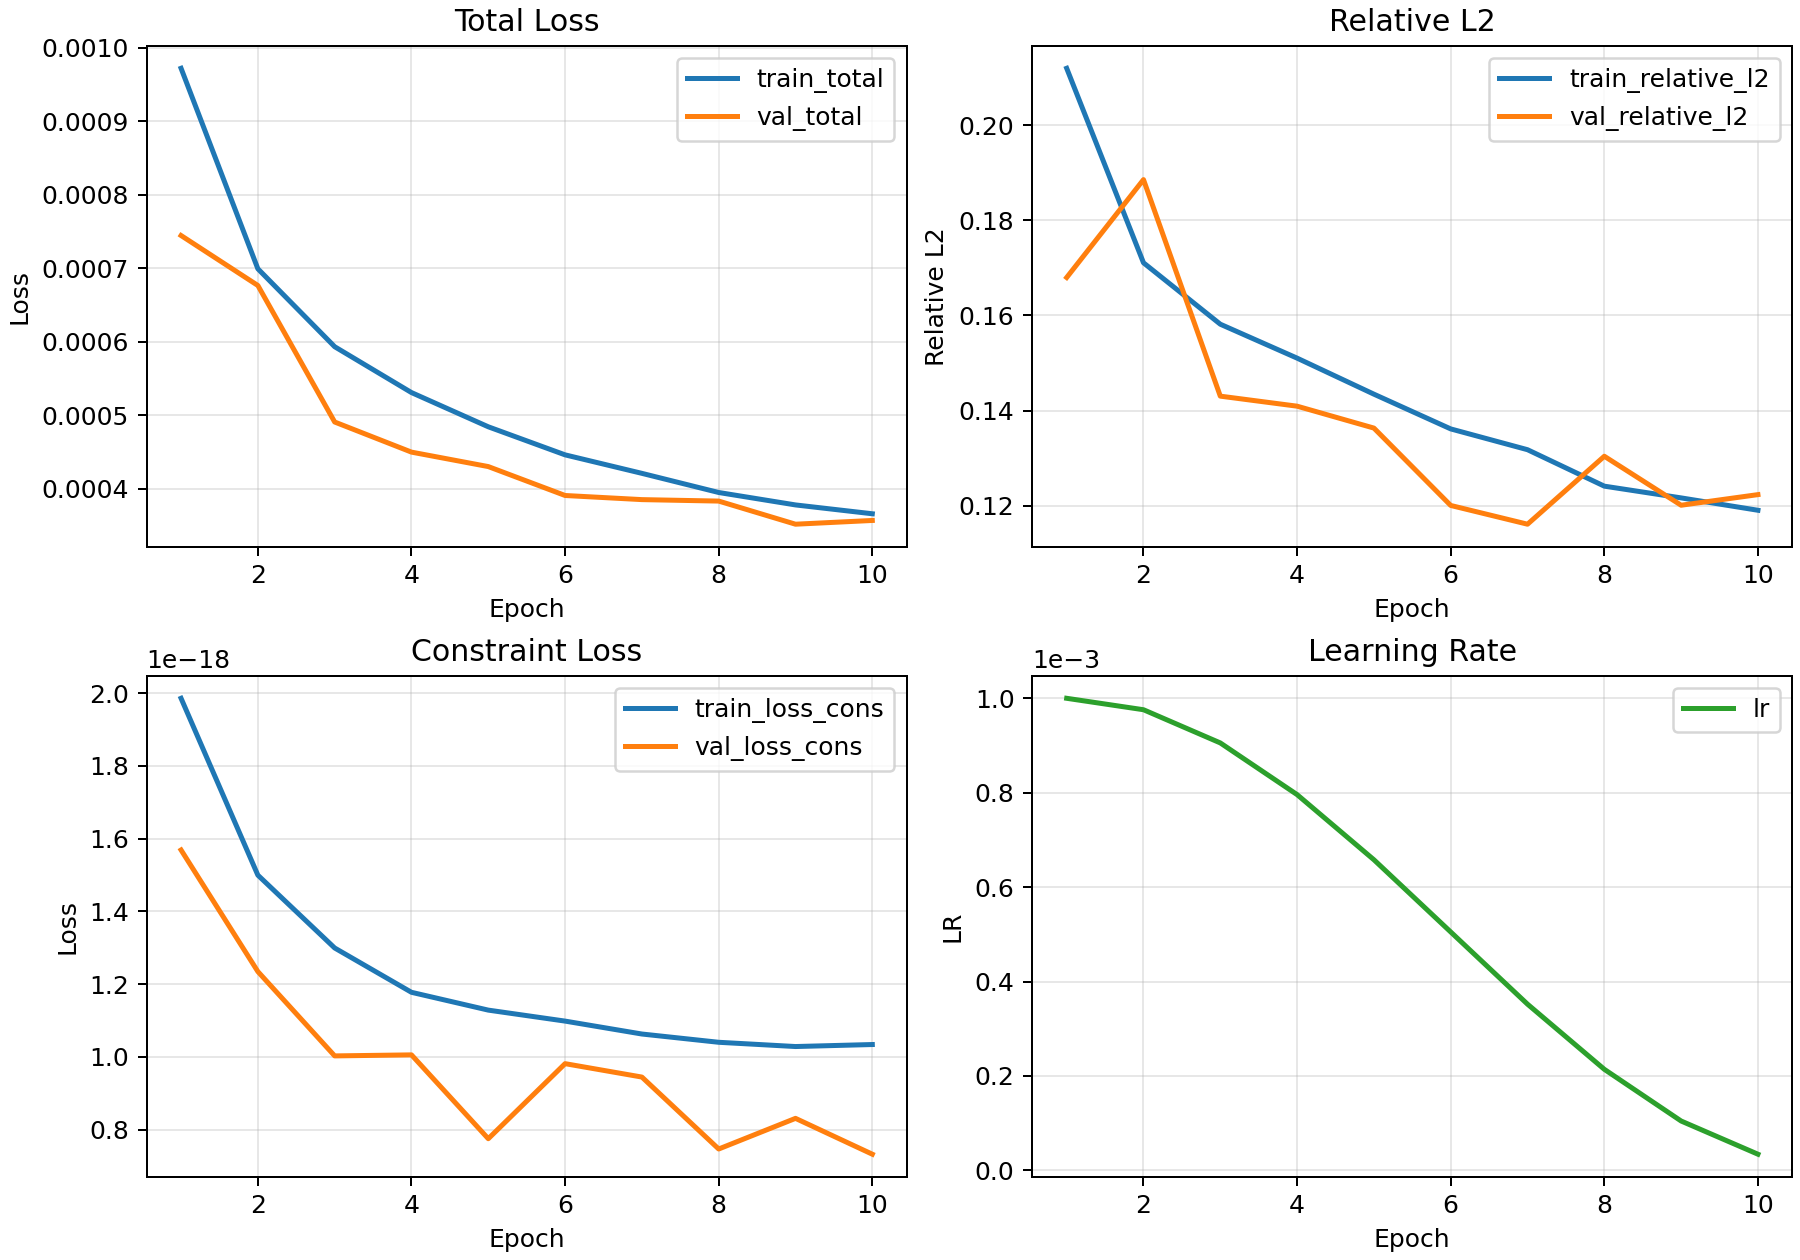
\includegraphics[width=\linewidth]{figures/training_curves_kernel.png}

    \column{0.40\textwidth}
      \begin{table}
        \small
        \begin{tabular}{@{}lcc@{}}
          \toprule
          指标 & Kernel & MLP \\
          \midrule
          relative L2 & 0.1201 & 0.1791 \\
          global $L_\infty$ & 0.1969 & 0.2540 \\
          neg. fraction & 0.0464 & 0.0776 \\
          mean cond($M$) & 646.3 & 584.5 \\
          \bottomrule
        \end{tabular}
      \end{table}

      \vspace{0.6em}
      \begin{alertblock}{结论}
        在当前 production run 上，\\
        kernel backbone 相比 MLP baseline\\
        得到了更低的 relative L2 与更低的负值比例。
      \end{alertblock}
  \end{columns}
\end{frame}

\begin{frame}{首轮结果：对比与可视化}
  \begin{columns}[T,onlytextwidth]
    \column{0.56\textwidth}
      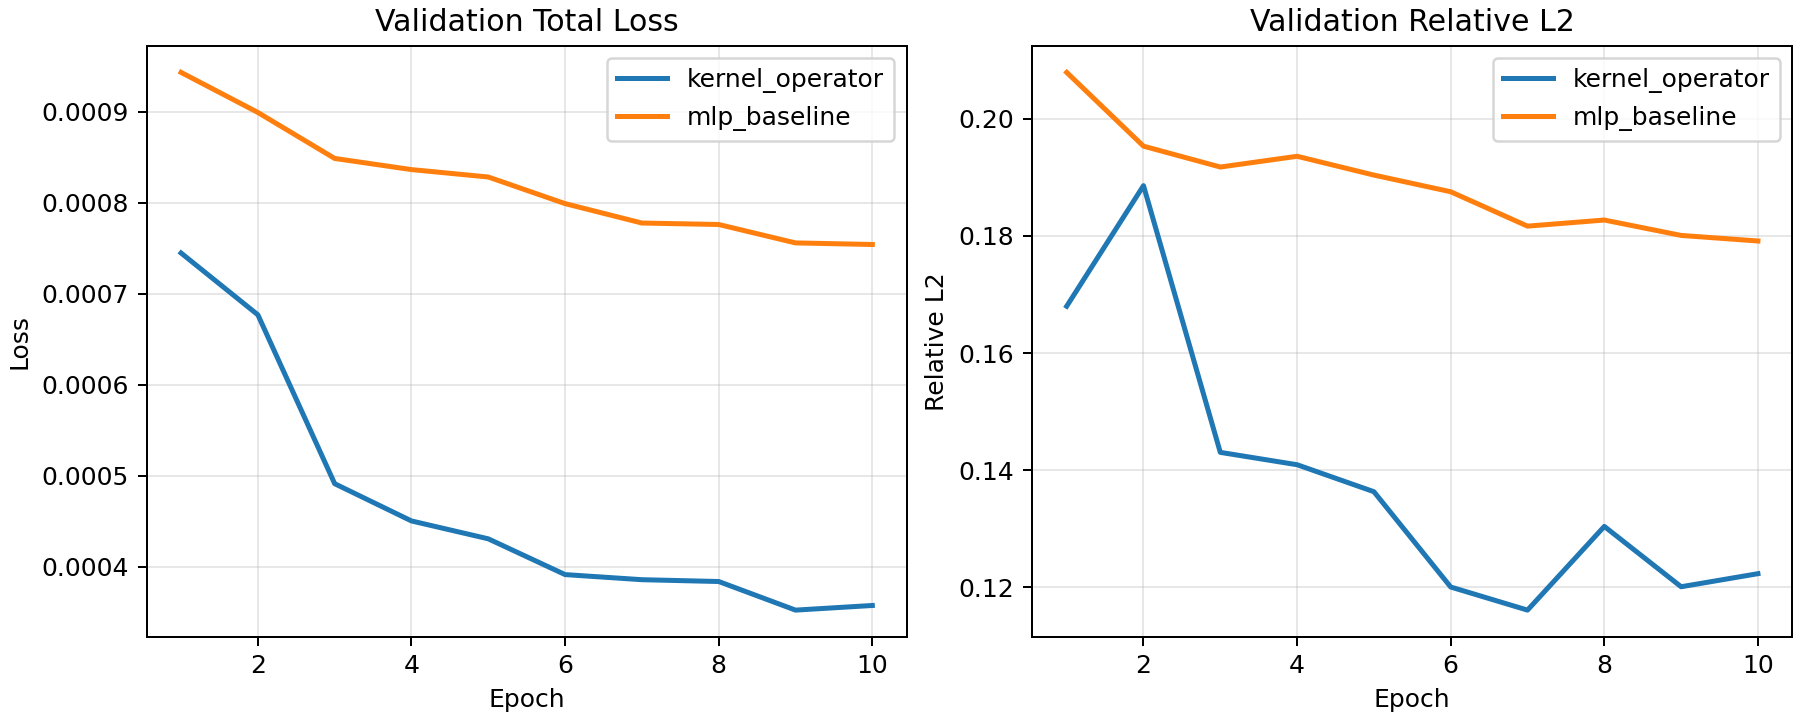
\includegraphics[width=\linewidth]{figures/comparison_kernel_vs_mlp.png}

    \column{0.40\textwidth}
      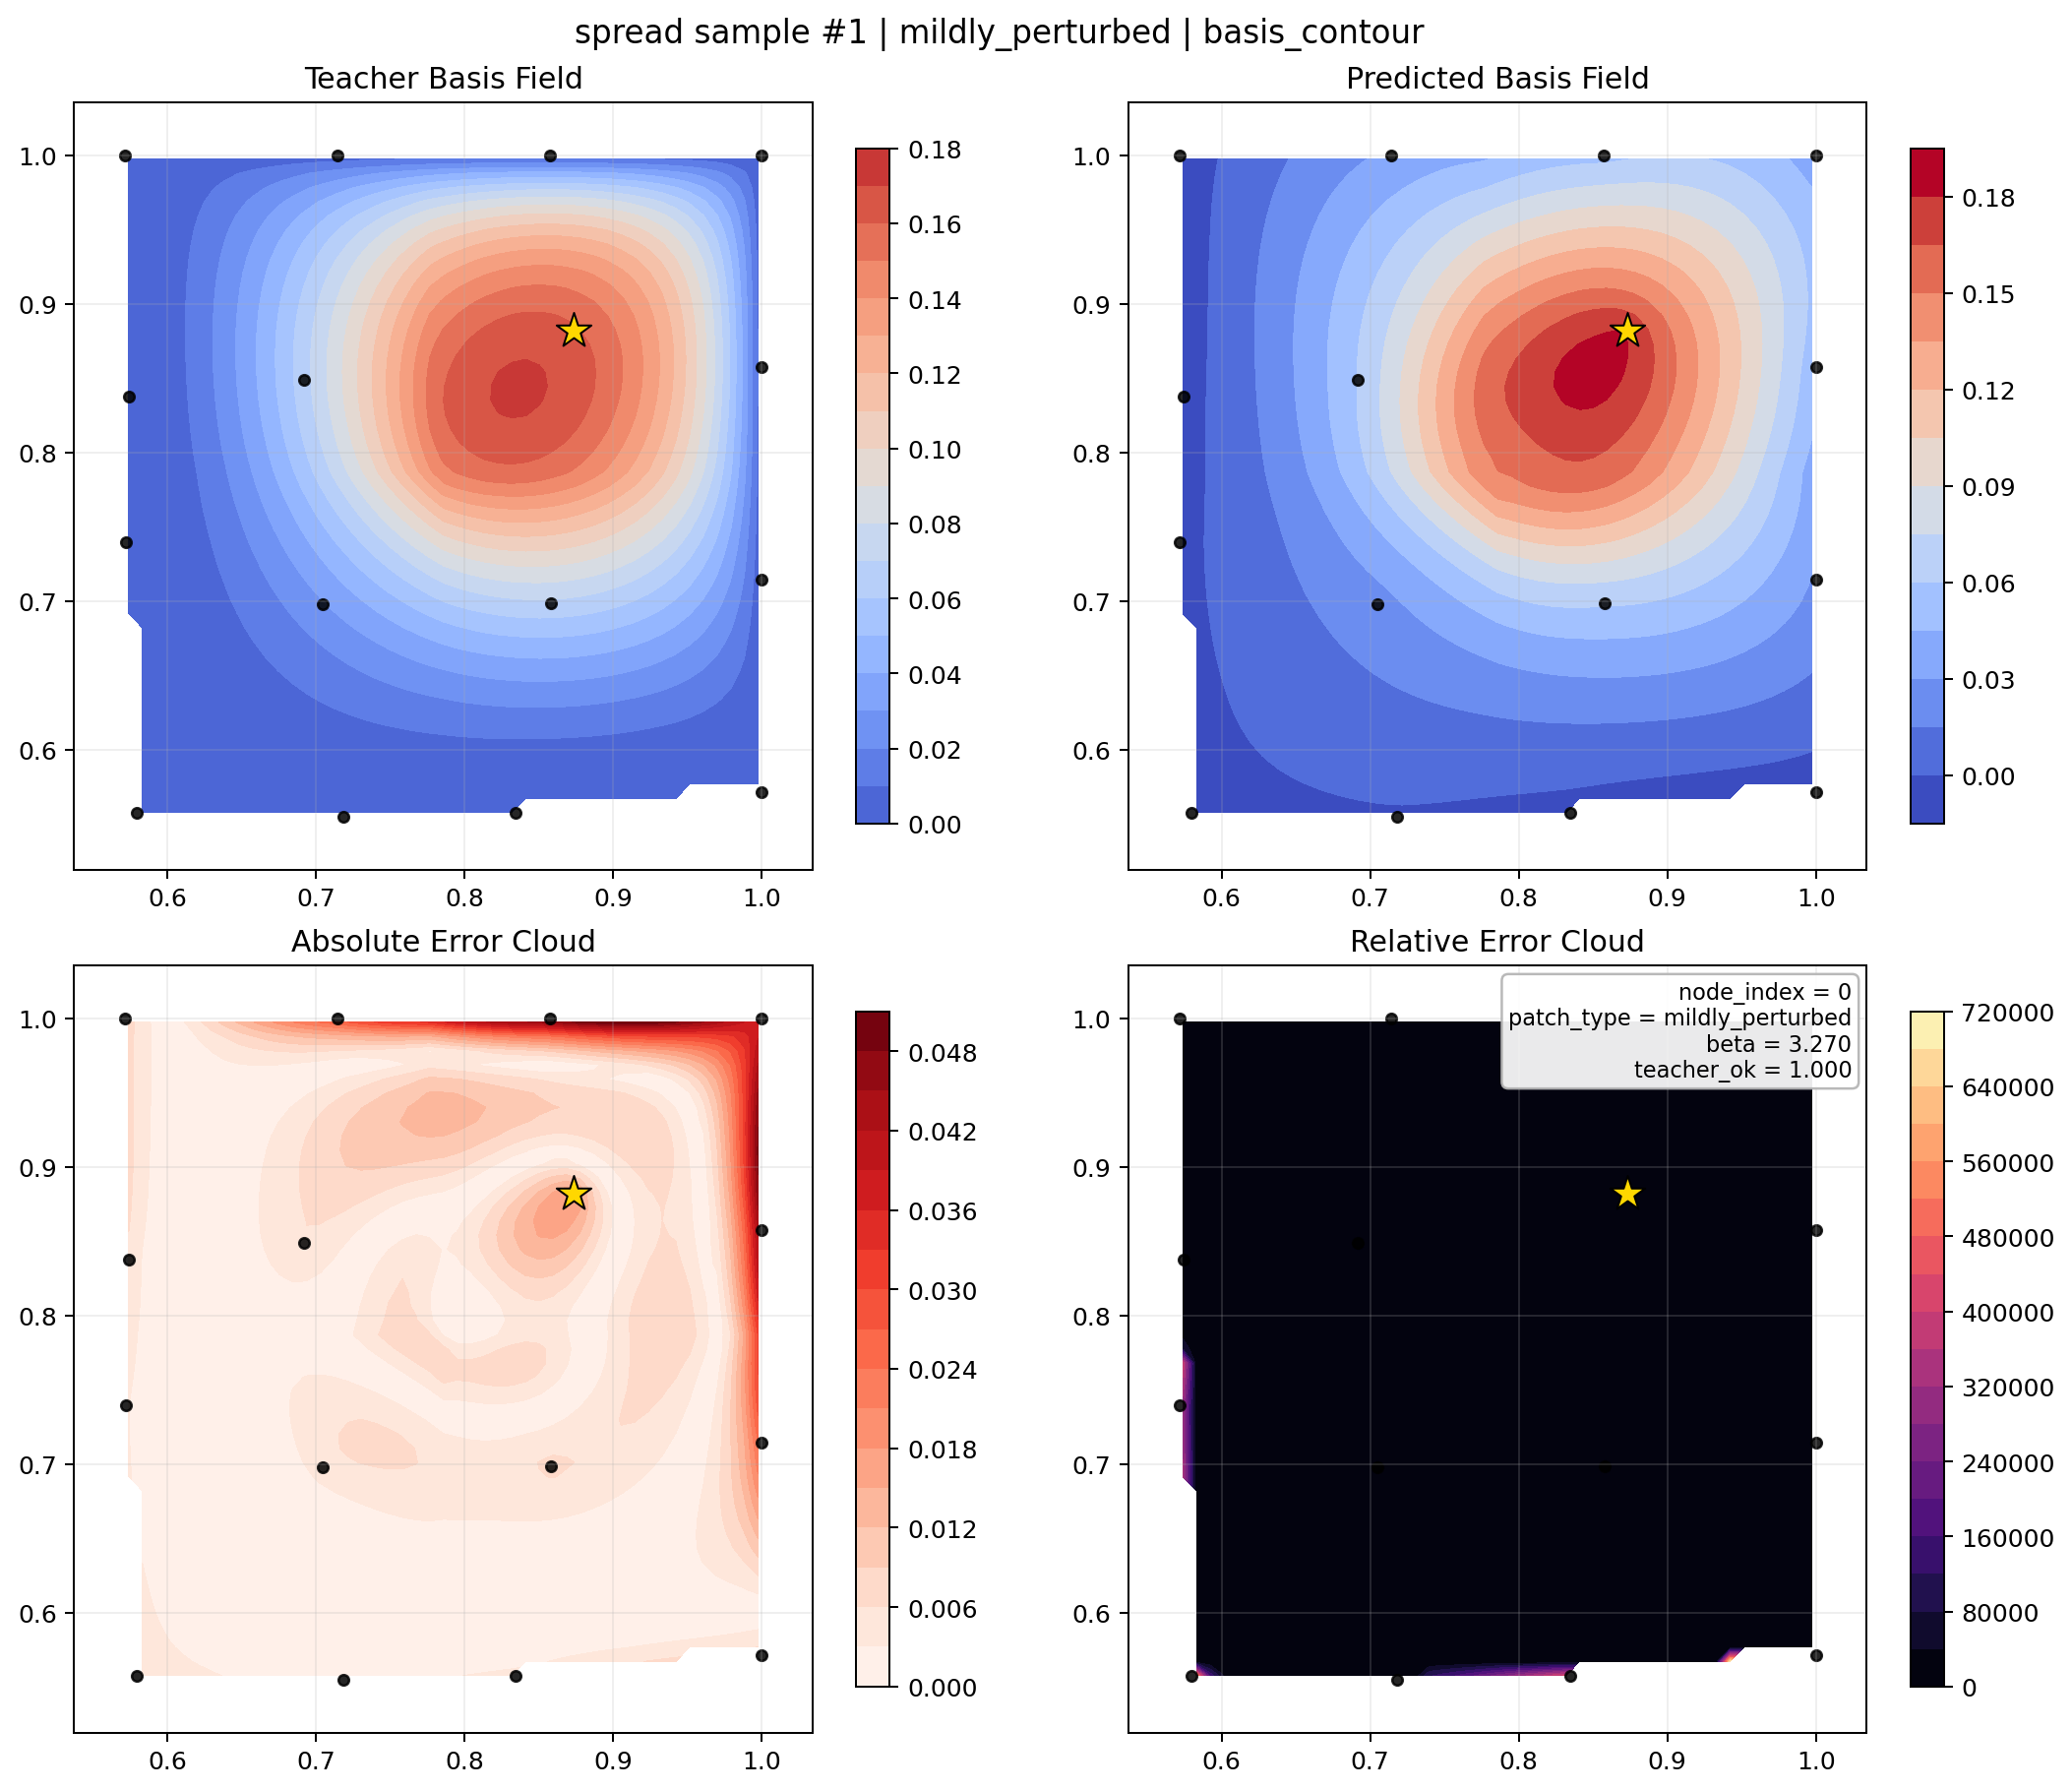
\includegraphics[width=\linewidth]{figures/basis_contour_good.png}

      \vspace{0.5em}
      \small
      左图：kernel vs MLP 总体对比\\
      右图：较好 patch 上的 basis contour
  \end{columns}
\end{frame}

\begin{frame}{误差模式：代表性难例}
  \begin{columns}[T,onlytextwidth]
    \column{0.60\textwidth}
      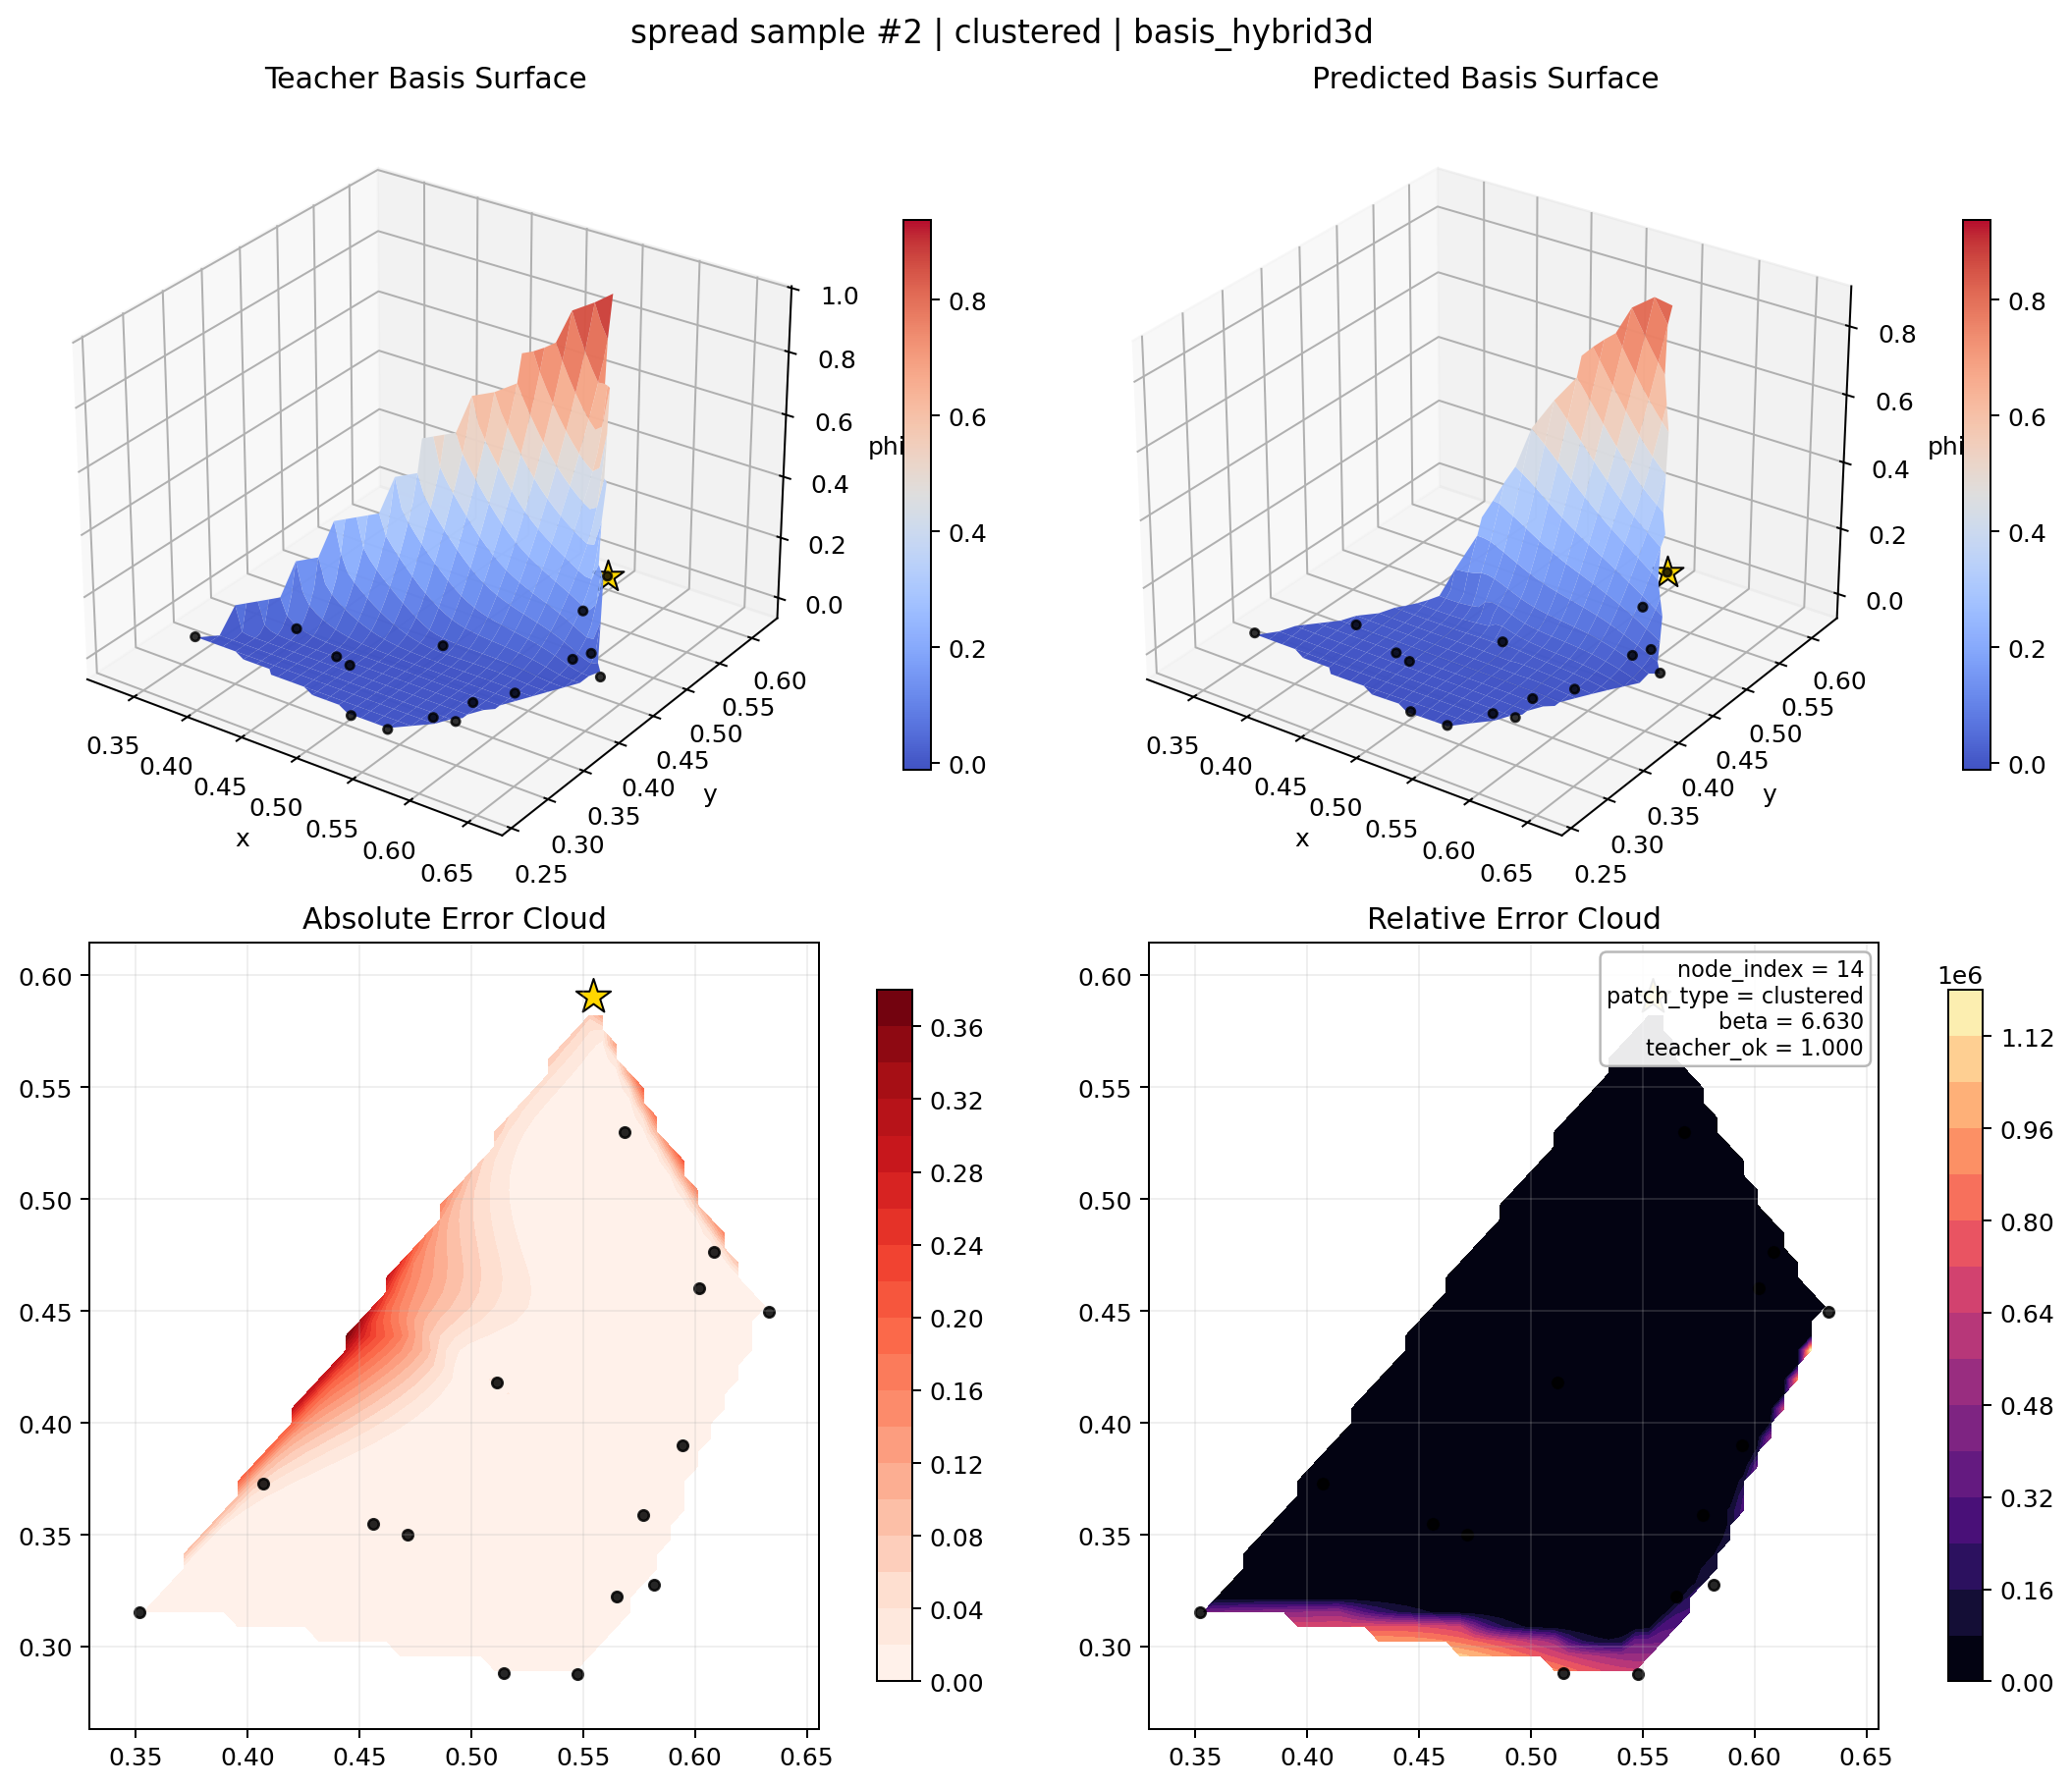
\includegraphics[width=\linewidth]{figures/basis_hybrid3d_hardcase.png}

    \column{0.36\textwidth}
      \begin{block}{观察}
        \begin{itemize}
          \item clustered / truncated patch 仍是主要难点
          \item hard case 上云图误差仍有局部集中区
          \item 但结构约束指标整体保持稳定
        \end{itemize}
      \end{block}

      \begin{alertblock}{解释}
        现在的图里 relative error cloud 已做\\
        \[
        \frac{|\phi-\phi^{\mathrm{ref}}|}
        {\max(|\phi^{\mathrm{ref}}|,\varepsilon)}
        \]
        的 \alert{floor mask + clip}，\\
        避免边界处因分母接近 0 而失真爆炸。
      \end{alertblock}
  \end{columns}
\end{frame}

\begin{frame}{下一步}
  \begin{columns}[T,onlytextwidth]
    \column{0.49\textwidth}
      \begin{block}{方法侧}
        \begin{itemize}
          \item 继续检查 teacher prior 与 head locality 的一致性
          \item 做 head ablation，验证 B4 的实际收益
          \item 补 OOD patch / $\beta$ 评估
        \end{itemize}
      \end{block}
    \column{0.49\textwidth}
      \begin{block}{工程侧}
        \begin{itemize}
          \item 收口默认 artifacts 与 figures
          \item 继续优化 GPU 利用率
          \item 为论文与答辩沉淀统一图表入口
        \end{itemize}
      \end{block}
  \end{columns}

  \vspace{0.8em}
  \begin{center}
    \Large 当前阶段结论：\alert{方法闭环已建立，kernel backbone 已显示出明确优势，但难例 patch 仍需进一步攻关。}
  \end{center}
\end{frame}

\begin{frame}[standout]
  Questions?
\end{frame}

\end{document}
